%% The following has to be declared in all included files

\fancyfoot[C]{\mbox{\texttt{3\_irreps.tex}}}
\fancyfoot[RO,LE]{\mbox{$$Revision: 1.9 $$}}
\fancyfoot[LO,RE]{\mbox{$$Date: 2011-10-24  $$}}
% Correcting the title chapter page
\fancypagestyle{plain}{%
    \fancyhf{}
    \fancyhead[RO,LE]{\bfseries \thepage}
    \fancyhead[CO]{\rightmark}
    \fancyhead[CE]{\leftmark}
     \fancyfoot[C]{\texttt{3\_irreps.tex}}
     \fancyfoot[RO,LE]{\mbox{$$Revision: 1.9 $$}}
     \fancyfoot[LO,RE]{\mbox{$$Date: 2011-10-24  $$}}
    \renewcommand{\headrulewidth}{0.4pt}
    \renewcommand{\footrulewidth}{0.4pt}}


\chapter{Svojstva ireducibilnih reprezentacija}

\section{Schurove leme i relacije ortogonalnosti}

Sva ključna svojstva ireducibilnih reprezentacija slijede iz 
dvije Schurove leme.

\begin{teorem}[Prva Schurova lema]
Neka operator S povezuje dvije  ireducibilne
reprezentacije $\Gamma=\{D(g)\}$ i $\Gamma'=\{D'(g)\}$:
\begin{displaymath}
  SD(g)=D'(g)S  \quad \forall g\in G  \;.
\end{displaymath}
Tada je ili $S=0$ ili je $S$ invertibilan i imamo
\begin{displaymath}
D(g)=S^{-1}D'(g)S
\end{displaymath}
tj. dvije su reprezentacije ekvivalentne. (Mogućnost
da je $S$ singularan, ali ne i nul-operator je isključena.)
\end{teorem}

\centerline{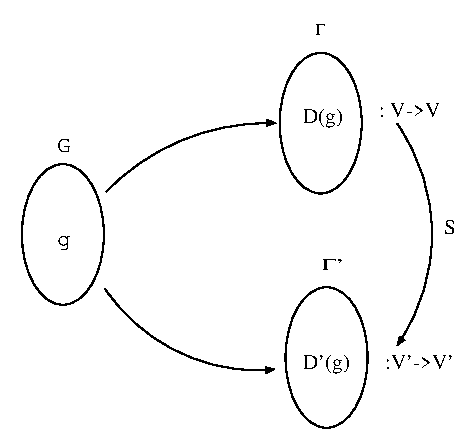
\includegraphics[scale=0.8]{pics/schur.eps}}

\textbf{Dokaz}$^{*}$: 

-$S\vec{x}=\vec{y}\in V'$

-$S(V)=\{S\vec{x} \td x \in V \}$ je potprostor od $V'$ (Sva potrebna svojstva
  $S(V)$  nasljeđuje od  $V'$, a zatvorenost i egzistencija inverza su 
 posljedice linearnosti operatora $S$.)


-$D'(g)S\vec{x}=SD(g)\vec{x} \in S(V) \imp  S(V)$ je invarijantni
   potprostor od $V'$

-Kako je $\{D'(g)\}$ IRREP, $\imp S(V)=\{\vec{0'}\}$ ili $S(V)=V'$

\begin{enumerate}[1)]
\item $ S(V)=\{\vec{0'}\} \imp  S=0$

\item $S(V)=V'$ tj. $S$ je surjekcija -- Promotrimo Ker($S$) 

  - Ker($S$) je potprostor od $V$ (trivijalno, linearnost od $S$)

  - $\vec{k}\in$Ker($S$) $\imp S D(g) \vec{k} = D'(g)S\vec{k} =
    \vec{0'} \imp D\vec{k} \in $Ker($S$) $\imp$ Ker($S$) je
    invarijantni potprostor; $\{D(g)\}$ je IRREP $\imp
    $Ker($S$)$=\{\vec{0}\}$ ili Ker($S$)=$V$

  - Ker($S$)$=V$ ne može biti jer onda ne bi bilo $S(V)=V'$ već
      $S(V)=\vec{0'}$

  - $\imp $Ker($S$)$=\{\vec{0}\}$ pa je $S$ i injekcija te ima inverz
    $\imp D(g)=S^{-1}D'(g)S$


\end{enumerate}

\begin{teorem}[Druga Schurova lema]
Operator koji komutira sa svim operatorima neke ireducibilne 
reprezentacije je nužno proporcionalan jediničnom operatoru
(identiteti).
\begin{displaymath}
  D(g)S=SD(g) \quad \forall g\in G \imp S = \lambda \Eins
\end{displaymath}
\end{teorem}

\textbf{Dokaz:}$^{*}$ \\

- $\exists \vec{x}\neq\vec{0} \td S\vec{x}=\lambda\vec{x}$ (Egzistencija barem
  jednog takvog vektora je ne sasvim trivijalan rezultat iz linearne algebre:
  Egzistenciju garantira postojanje rješenja karakteristične
  jednadžbe $\det(S - \lambda \Eins)=0$, što je opet garantirano fundamentalnim
   teoremom algebre, za $\lambda \in \mathbb{C}$.)

- $\imp (S-\lambda\Eins)\vec{x}=0 \imp (S-\lambda\Eins)$
  je singularna matrica (neki vektor $\neq \vec{0}$ preslikava u
  $\vec{0'}$ pa nije injekcija)

- No, $[S-\lambda\Eins, D(g)]=0 \imp S-\lambda\Eins =0$
  po prvoj lemi. Slijedi $S=\lambda\Eins$.




\subsubsection*{Relacije ortogonalnosti}
\label{sec:ortogonalnost}

Promotrimo sada dvije IRREPs: $\Gamma_{\alpha}$ i $\Gamma_{\beta}$.
Ako je $\alpha\neq\beta$ podrazumijevamo da su reprezentacije
neekvivalentne.

\begin{align*}
D^{(\alpha)} &: V^{(\alpha)} \to V^{(\alpha)} \\
D^{(\beta)}  &: V^{(\beta)}  \to V^{(\beta)} \\
A          &: V^{(\beta)} \to V^{(\alpha)} \qquad \text{proizvoljni operator}
\end{align*}

Definirajmo matricu:
\begin{equation*}
B\equiv \sum_{g\in G} D^{(\alpha)}(g) A D^{(\beta)}(g^{-1}) \;,
\end{equation*}
gdje je $A$ proizvoljna matrica odgovarajućih dimenzija.
Pokazat ćemo da $B$ zadovoljava pretpostavke Schurovih lema.
Uzimimo proizvoljni element $h\in G$. Tada vrijedi:
\begin{equation*}
\begin{split}
 D^{(\alpha)}(h)B &= \sum_g D^{(\alpha)}(h) D^{(\alpha)}(g) A
    D^{(\beta)}(g^{-1}) \\
&= \sum_g D^{(\alpha)}(hg) A D^{(\beta)}(g^{-1}) \\
&= ( \textrm{zamjenom}\; hg\equiv g' \, , \; g^{-1}=g'^{-1}h ) \\
&= \sum_{g'} D^{(\alpha)}(g') A D^{(\beta)}(g'^{-1}h) \\
&= \sum_{g'} D^{(\alpha)}(g') A D^{(\beta)}(g'^{-1}) D^{(\beta)}(h) \\
&= B D^{(\beta)}(h)
\end{split}
\end{equation*}

U slučaju $\alpha\neq\beta$ ($\Gamma_\alpha$ i $\Gamma_\beta$ nisu 
ekvivalentne),
iz prve Schurove leme slijedi da je $B=0$. Ako je pak $\alpha=\beta$, tj.
$D^{(\alpha)}(h)=D^{(\beta)}(h)$ onda iz druge Schurove leme
slijedi $B=\lambda \Eins$.
Ove se dvije tvrdnje mogu kompaktno ujediniti u relaciju
\begin{displaymath}
  B = \sum_g D^{(\alpha)}(g) A D^{(\beta)}(g^{-1}) =
 \lambda^{(\alpha)}_A \delta^{\alpha\beta} \Eins \;,
\end{displaymath}
odnosno, po komponentama,
\begin{displaymath}
\sum_g D^{(\alpha)}_{ir}(g) A_{rs} D^{(\beta)}_{sl}(g^{-1})
 = \lambda_{A}^{(\alpha)} \delta^{\alpha\beta} \Eins_{il}
\end{displaymath}

$A$ je bila proizvoljna matrica. Uzmimo sada konkretnije na mjesto $A$
matricu $A^{(j,k)}$ koja je svugdje nula osim što joj je
element $A^{(j,k)}_{jk}=1$:
\begin{displaymath}
 A^{(j,k)}=
\begin{array}{cc}
 & \cdots k \cdots \\
        \begin{array}{c}
         \cdot \\ \cdot \\ j \\ \cdot \\ \cdot \\ \cdot 
        \end{array}
 & 
\begin{pmatrix}
  & \cdot & \\
  & \cdot & \\
 \cdots & 1  & \cdots \\
  & \cdot & \\
  & \cdot & \\
  & \cdot & \\
\end{pmatrix}
\end{array}
\end{displaymath}
\begin{displaymath}
A^{(j,k)}_{rs}=\delta_{rj}\delta{sk} 
\end{displaymath}

Upotrebom te matrice u gornjoj relaciji dobivamo
\begin{displaymath}
\sum_g D^{(\alpha)}_{ij}(g) D^{(\beta)}_{kl}(g^{-1}) = 
 \lambda^{(\alpha)}_{jk} \delta^{\alpha\beta} \Eins_{il} \;.
\end{displaymath}

Sada treba odrediti $\lambda_{jk}$. 
Stavimo ovdje $\alpha =\beta$ i uzmimo trag po $il$ indeksima
\begin{displaymath}
\sum_g D^{(\alpha)}_{ij}(g) D^{(\alpha)}_{ki}(g^{-1}) = 
 \lambda^{(\alpha)}_{jk} \delta^{\alpha\alpha}\, \textrm{dim}(V^{(\alpha)})
 \equiv \lambda^{(\alpha)}_{jk} d_{\alpha}
\end{displaymath}
S druge strane, to je također jednako
\begin{displaymath}
 \sum_g D(g^{-1}g)_{kj}= \sum_g \Eins_{kj} = \delta_{kj} \sum_g 
 = \delta_{kj} n \;.
\end{displaymath}
Ovdje je $n$ red grupe G.
Slijedi da je
\begin{displaymath}
\lambda^{(\alpha)}_{jk}= \frac{n}{d_{\alpha}}\delta_{kj} \;,
\end{displaymath}
što daje \emph{temeljni teorem o ortogonalnosti} matrica ireducibilnih
reprezentacija:
\begin{displaymath}
\sum_g D^{(\alpha)}_{ij}(g) D^{(\beta)}_{kl}(g^{-1}) =
 \frac{n}{d_{\alpha}}\delta^{\alpha\beta}\delta_{il}\delta_{kj} \;.
\end{displaymath}



Nadalje, uvijek možemo uzeti da je $D^{(\alpha)}(g)$ unitarna matrica
\begin{displaymath}
\sum_g D^{(\alpha)}_{ij}(g) D^{(\beta)}_{lk}(g)^* =
 \frac{n}{d_{\alpha}}\delta^{\alpha\beta}\delta_{il}\delta_{kj} \;.
\end{displaymath}
Stavimo ovdje $\alpha=\beta$ i promotrimo skup od $d^{2}_\alpha$ vektora
$\vec{x}_{ij}$ iz novog $n$-dimenzionalnog vektorskog prostora,  čije
su komponente dane komponentama matrica reprezentacije:
\begin{displaymath}
\vec{x}_{ij} \equiv
(D^{(\alpha)}_{ij}(g_1), D^{(\alpha)}_{ij}(g_2), \ldots, 
D^{(\alpha)}_{ij}(g_n))
\end{displaymath}
(Ne miješati ovaj
prostor s $V^{\alpha}$ koji je dimenzije $d_\alpha$!) Zbog
\begin{displaymath}
\sum_g D^{(\alpha)}_{ij}(g) D^{(\alpha)}_{lk}(g)^* = (\vec{x}_{lk},\vec{x}_{ij})
 =\frac{n}{d_{\alpha}}\delta_{il}\delta_{kj}
\end{displaymath}
vektori $\vec{x}_{ij}$ su međusobno ortogonalni.

Za neku drugu ireducibilnu reprezentaciju 
$\Gamma_{(\alpha')}$ imamo novih $d_{\alpha'}^{2}$
vektora  koji su ortogonalni međusobno, ali i obzirom na prvih
$d_{\alpha}^{2}$ vektora. Treća IRREP daje novih $d_{\alpha''}^{2}$ itd.
No, maksimalan broj ortogonalnih vektora u $n$-dimenzionalnom vektorskom
prostoru je $n$ 
\begin{displaymath}
\sum_{\alpha} d_{\alpha}^{2} \leq n  
\end{displaymath}
pa kako je svaka IRREP barem 1D imamo $\sum_{\alpha} d_\alpha \leq n$ tj.
broj IRREPsa je manji ili jednak broju elemenata grupe..

Štoviše, vrijedi (vidi literaturu):
\begin{displaymath}
\sum_{\alpha} d_{\alpha}^2 = n
\end{displaymath}

Da bismo odredili broj IRREPsa grupe, treba nam pojam \emph{karaktera}
reprezentacije.

\begin{definicija}[Karakter reprezentacije]
Karakter $\chi$ reprezentacije $\Gamma=\{D(g)\}$ grupe $G$ je skup
$\chi=\{\chi(g) = \Tr D(g) \td  g\in G\}$.
\end{definicija}

Svojstva:

- $\Tr S D(g) S^{-1} = \Tr D(g)$ - zbog cikličnosti traga
  $\imp$ ekvivalentne REP imaju iste karaktere

- Bez dokaza: vrijedi i obrat: isti karakteri $\imp$ ekvivalentne REP
  (Ali taj obrat se ne poopćuje na beskonačne kontinuirane grupe, osim
   ukoliko nisu kompaktne, vidi \cite{Cornwell84} p. 302)

- $\chi(g)=\Tr D(g) = \Tr D(h) D(g) D^{-1}(h) = \Tr D(hgh^{-1})$
  $\to$ konjugirani elementi imaju iste karaktere (Oprez: Treba
  razlikovati karakter reprezentacije $\chi$ od njegove komponente
  $\chi(g)$ koju isto često zovemo karakter --- karakter elementa.)

- za unitarnu REP $\chi(g^{-1}) = \Tr D(g^{-1})= \Tr D^{\dagger}
    = \chi^{*}(g)$


Teorem o ortogonalnosti  /$\delta_{ij}\delta_{kl}$
\begin{displaymath}
\sum_g \chi^{(\alpha)}(g) \chi^{(\beta)}(g)^* = 
\frac{n}{d_{\alpha}} \delta^{\alpha\beta} \delta_{ik}\delta_{ki} =
\frac{n}{d_{\alpha}} \delta^{\alpha\beta} d_{\alpha} =
n \delta^{\alpha\beta} 
\end{displaymath}

Definiramo li skalarni produkt karaktera
 \begin{displaymath}
(\chi, \phi) \equiv \frac{1}{n} \sum_g \chi(g) \phi(g)^* = (\phi, \chi) \;,
\end{displaymath}
imamo
\begin{displaymath}
(\chi^{(\alpha)}, \chi^{(\beta)}) = \delta^{\alpha\beta}
\end{displaymath}
tj. karakteri neekvivalentnih IRREPsa su ortonormirani.

Neka je sada $k_i$ broj elemenata u $i$-toj klasi konjugacije grupe $G$.
Tada, budući da su karakteri svih elemenata jedne klase konjugacije
isti imamo
\begin{displaymath}
(\chi^{(\alpha)}, \chi^{(\beta)})=\frac{1}{n} \sum_{i=1}^{k}  k_i
 \chi^{(\alpha)}_i \chi^{(\beta)*}_{i} = \delta^{\alpha\beta} \;.
\end{displaymath}
što je iskaz ortogonalnosti vektora u $k$-dimenzionalnom vektorskom
prostoru, gdje su sada vektori
\begin{displaymath}
\vec{\chi}^{(\alpha)} = (\chi^{(\alpha)}_1, \chi^{(\alpha)}_2, \ldots,
 \chi^{(\alpha)}_{k})
\end{displaymath}
Svaka IRREP daje jedan takav $k$-dimenzionalni vektor.
Istim logičkim slijedom kao i ranije ova ortogonalnost vodi na zaključak 
da je broj
IRREPsa  manji ili jednak broju klasa konjugacije. Štoviše, vrijedi
(vidi literaturu) ortogonalnost vektora:
\begin{displaymath}
\vec{\chi}_i = (\chi^{(\alpha)}_i, \chi^{(\beta)}_i, \ldots)
\end{displaymath}
tj.
\begin{displaymath}
\frac{1}{n} \sum_{\alpha} k_i \chi^{(\alpha)}_i \chi^{(\alpha)*}_j =
\delta_{ij}
\end{displaymath}
što na isti način daje suprotnu nejednakost da je broj klasa konjugacije manji
ili jednak broju IRREPsa.
Dakle, broj IRREPsa je upravo jednak broju klasa konjugacije!

\section{Tablice karaktera}

\emph{Tablica karaktera} neke grupe je tablica strukture

\begin{tabular}{c|c}
  & Klase konjugacije \\ \hline
\begin{turn}{90} IRREPs \end{turn} & {\Huge $\chi$}
\end{tabular}

Ona često daje dovoljno informacija za praktične primjene, a može
se pomoću slijedećih pravila konstruirati i bez eksplicitnog
poznavanja matrica reprezentacije.

\subsection*{Pravila za konstrukciju tablice karaktera}

\begin{enumerate}

\item Broj ireducibilnih reprezentacija jednak je broju klasa konjugacije 
  grupe. Iz ovoga slijedi da tablica ima jednak broj redova i stupaca. 
  Broj klasa pronalazimo "pješke," analizom grupe.

\item $\sum_{\alpha} d_{\alpha}^2 = n$ često ima jedinstveno rješenje koje
  određuje dimenzionalnosti $d_{\alpha}$ ireducibilnih reprezentacija.

\item Jedinični element grupe je klasa za sebe, a reprezentiran je uvijek
  jediničnom matricom $D^{(\alpha)}(e)=\Eins$ čiji je 
   karakter $\chi^{(\alpha)}(e)=d_{\alpha}$.
  Ovo određuje jedan (konvencionalno prvi) stupac tablice.

\item Uvijek postoji trivijalna jednodimenzionalna ireducibilna
   reprezentacija  $D(g)=\chi(g)=1  \;
    \forall g\in G$.
  Dakle jedan red (konvencionalno prvi) se sastoji od samih jedinica.

\item Za jednodimenzionalne reprezentacije vrijedi $D(g)=\chi(g)$ pa
  sami karakteri reprezentiraju grupu i njihovo množenje mora odražavati
  množenje odgovarajućih elemenata grupe.

\item  \[\sum_{i=1}^{k} k_{i} \chi^{(\alpha)}_{i} \chi^{(\beta) *}_{i} =
    n \delta^{\alpha\beta}\] 
(\emph{Redovi} tablice su ortogonalni i, kad se uzmu u obzir težinski
  faktori $k_i$, normirani su na $n$)

\item  \[\sum_{\alpha=1}^{k} k_{i} \chi^{(\alpha)}_{i} \chi^{(\alpha) *}_{j} =
    n \delta_{ij} \] 
(\emph{Stupci} tablice su ortogonalni i, kad se uzmu u obzir težinski
  faktori $k_i$, normirani su na $n$)

\end{enumerate}

Pravila je najbolje primjenjivati po redu jer su ona s većim rednim
brojem teža za primjenu i rjeđe nužna za kompletiranje tablice.


\begin{primjer}[$D_3$]

Klase konjugacije su (vidi raniji primjer iz odjeljka 1.2):

$K_1=\{e\}$

$K_2 = \{c, c^2\}$

$K_3 = \{ b, bc, bc^2 \}$

1. pravilo $\imp$ 3 IRREPsa

2. $\imp$ $\sum_{\alpha=1}^{3} d_{\alpha}^2 = d_{1}^2 + d_{2}^2
   + d_{3}^2 = n = 6 $ \\
     $\imp d_1 = d_2 =1, d_3=2 $

3. $\imp$ prvi stupac: 1, 1, 2

4. $\imp$ prvi red: 1, 1, 1

\begin{tabular}{c|ccc}
  & $K_1$ & 2$K_2$  & 3$K_3$ \\ \hline
$\Gamma_1$ &   &  &   \\
$\Gamma_2$ &   &  &   \\
 $\Gamma_3$  &   &  &  
\end{tabular}

5. $\chi^{(2)}(b)\chi^{(2)}(c)=\chi^{(2)}(bc), \chi(b)=\chi(bc)$ \\
  $\imp \chi(c)=1$ \\
  $\chi(b)\chi(b)=\chi(b^2)=\chi(e)=1 \imp \chi(b)=\pm 1 $

6. Kad bi bilo $\chi^{(2)}(b)=1$ prva dva reda bi bila jednaka, a ne
   ortogonalna. $\imp \chi^{(2)}(b)=-1$.

   $\sum_{i=1}^{3} k_{i} \chi^{(3)}_{i} \chi^{(1) *}_{i} =
      2+2a+3b=0$ \\
   $\sum_{i=1}^{3} k_{i} \chi^{(3)}_{i} \chi^{(2) *}_{i} =
      2+2a-3b=0$ \\
   $\imp a=-1, b=0$

- obično se za označavanje IRREPsa i klasa koriste kristalografske
   oznake iz priloga.
 

\begin{tabular}{c|ccc}
  & E & 2$C_3$  & 3$C_2$ \\ \hline
$A_1$ & 1 & 1& 1 \\
$A_2$ & 1 & 1&-1 \\
 $E$  & 2 &-1& 0
\end{tabular}

\end{primjer}

\begin{primjer}[$C_3$]

Abelova grupa, svaki element je klasa : $e, c, c^2$

Dakle, tri klase i $d_{1}^2+d_{2}^2+d_{3}^2 = n =3$ pa su
sve tri IRREP 1D.

Prvi red i prvi stupac: sve jedinice

5. pravilo: $\chi(c)^3=\chi(c^3)=\chi(e)=1 \imp \chi(c)=
  \exp(2\pi i k/3), k=0, 1, 2 $

$\chi(c)=1, \omega=e^{2\pi i/3}, \omega^2$

\begin{tabular}{c|ccc}
  & E & $c=C_3$  & $c^2=C_{3}^2$ \\ \hline
$D^{(1)}$ & 1 & 1& 1 \\
$D^{(2)}$ & 1 & $\omega$ &$\omega^2$  \\
 $D^{(3)}$  & 1 &$\omega^2$ & $\omega$ 
\end{tabular}

- provjeriti ortogonalnost

$\omega^2 = \omega^* \imp$ $D^{(2)}$ i $D^{(3)}$ su kompleksno
konjugirane reprezentacije. (Sve smo to već vidjeli ranije u
vježbama.)


Zgodno je uočiti da neabelovska grupa $D_3$ ima i dvodimenzionalnu, dakle matričnu,
ireduciblinu reprezentaciju. To je logično jer neabelovsko svojstvo ne može biti
vjerno reprezentirano jednodimenzionalnim reperezentacijama.
\end{primjer}

\section{Dekompozicija reducibilnih reprezentacija}

Uzmimo neku reprezentaciju $\Gamma$. Po definiciji,
\begin{displaymath}
  \Gamma = \Gamma^{(1)}\oplus\Gamma^{(2)}\oplus\cdots =
     \sum_{\alpha}  a_{\alpha} \Gamma^{\alpha}
\end{displaymath}
gdje su $\Gamma^{\alpha}$ IRREPsi i
gdje je $a_{\alpha}$ \emph{multiplicitet} (broj pojavljivanja) 
IRREPsa $\Gamma^{\alpha}$ u $\Gamma$.


Tr / $ \imp  \chi_i = \sum_{\alpha}  a_{\alpha} \chi^{(\alpha)}_i \quad 
  \forall i$

$\sum_{i=1}^{k} k_i \chi^{(\beta)*}_i /  \imp $

$\sum_{i=1}^{k} k_i \chi_i \chi^{(\beta)*}_i =
\sum_{\alpha}  a_{\alpha} \sum_{i=1}^{k} k_i\chi^{(\alpha)}_i \chi^{(\beta)*}_i
=\sum_{\alpha}  a_{\alpha} n \delta^{\alpha \beta} = n a_{\beta} $


\begin{displaymath}
a_{\alpha} = \frac{1}{n} \sum_{i=1}^{k}  k_i \chi_i \chi^{(\alpha)*}_i
= (\chi^{(\alpha)}, \chi)
\end{displaymath}

\begin{primjer}[REP $\Gamma_V$ od $D_3$ na 3D euklidskom prostoru]
Pod $\Gamma_V$ misli se "vektorska" REP, tj. REP koja djeluje
na pravim 3D vektorima, za razliku od "nepravih" aksijalnih pseudovektora.
$D^{V}(e)=\textrm{diag}(1,1,1)$
\begin{displaymath}
D^{V}(c)=\left(
\begin{array}{ccc}
-1/2 & -\sqrt{3}/2 & 0 \\
\sqrt{3}/2 & -1/2 & 0 \\
0 & 0 & 1
\end{array}\right)
D^{V}(b)=\left(
\begin{array}{ccc}
-1 & 0 & 0 \\
0 & 1 & 0 \\
0 & 0 & -1
\end{array}\right) \textrm{ - rotacija za $\pi$ oko y}
\end{displaymath}
... je reducibilna reprezentacija. Koji je njen rastav na IRREPse?
$\chi=(3,0,-1)$

$a_{A_1} = (\chi, \chi^{(A_1)})=\frac{1}{n}\sum_{i=1}^{3} k_i \chi_i \chi^{(A_1)*}_i
 = \frac{1}{6}(1\cdot 3\cdot 1 + 2\cdot 0\cdot 1 + 3\cdot (-1) \cdot 1)=0$

$a_{A_2} = (\chi, \chi^{(A_2)})
=\frac{1}{6}(1\cdot 3\cdot 1 + 2\cdot 0\cdot 1 + 3\cdot (-1)\cdot(-1))=1$

$a_{E} = (\chi, \chi^{(E)})
=\frac{1}{6}(1\cdot 3\cdot 2 + 2\cdot 0\cdot (-1) + 3\cdot (-1)\cdot 0)=1$

$\Gamma_V  = A_2 \oplus E $

Koji su invarijantni potprostori?

$V^{(A_2)}$ je očito razapet vektorom $\hat{\vec{z}}$, a $\hat{\vec{x}}$ i
$\hat{\vec{y}}$ razapinju 2D potprostor $V^{(E)}$. (Primijetite razliku
prema $C_3$ kod koje je svaki vektor $\vec{v}=a\hat{\vec{z}}$ invarijantan.
$\to$ dipolni momenti.)
\end{primjer}


Direktan zbroj dviju IRREPsa je po definiciji reducibilna REP.
Što je s direktnim produktom?

Pokazali smo ranije da je direktan produkt dviju reprezentacija
$\Gamma^{(1)} \otimes \Gamma^{(2)}$ grupe G također reprezentacija
grupe G. Ona je u općenitom slučaju reducibilna:

\begin{displaymath}
  \Gamma^{(\alpha)}\otimes\Gamma^{(\beta)} =
  \sum \oplus\: a_{\gamma}\Gamma^{(\gamma)} \quad
   \textrm{ - Clebsch-Gordanov razvoj }
\end{displaymath}


Karakter direktnog produkta je produkt karaktera (očito ako pogledamo
matrični izgled direktnog produkta).$\imp$
\begin{displaymath}
a_{\gamma}  = (\chi^{(\gamma)}, \chi^{(\alpha)}\chi^{(\beta)}) \quad
\end{displaymath}

\begin{primjer}[$E\otimes E$ u $D_3$]
$\chi(E)=(2, -1, 0) \imp \chi(E\otimes E)=(4, 1, 0)$

$a_{A_1}=\frac{1}{6}(1\cdot 1\cdot 4+2\cdot 1\cdot 1+3\cdot 1\cdot 0)=1$

$a_{A_2}=\frac{1}{6}(1\cdot 1\cdot 4+2\cdot 1\cdot 1+3\cdot (-1)\cdot 0)=1$

$a_{E}=\frac{1}{6}(1\cdot 2\cdot 4+2\cdot (-1)\cdot 1+3\cdot 0\cdot 0)=1$

$E\otimes E = A_1 \oplus A_2 \oplus E $
\end{primjer}

\section{Primjena: \emph{Dipolni momenti kristala}}

Da bi kristal mogao imati permanentni magnetski ili električni dipolni
moment te veličine moraju biti invarijantne na grupu G simetrije
kristala.

Dipolni momenti su \emph{vektori} 3D euklidskog vektorskog prostora. Slijedi
da je za egzistenciju dipolnih momenata nužno postojanje vektora 
invarijantnih na djelovanje grupe.

Npr. za kristal s $C_3$ simetrijom vektor $\vec{P}$ je invarijantan i
to može biti smjer dipolnog  momenta takvog kristala. $\vec{P}\neq 0$
ne narušava $C_3$ simetriju.

\centerline{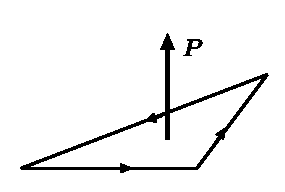
\includegraphics[scale=1.0]{pics/dipol.eps}}

S druge strane, veća $D_3$ simetrija ukida takvu mogućnost. $b$-rotacija
mijenja $\vec{P}\to-\vec{P}$ pa bi $\vec{P}\neq 0$ narušilo simetriju.

\centerline{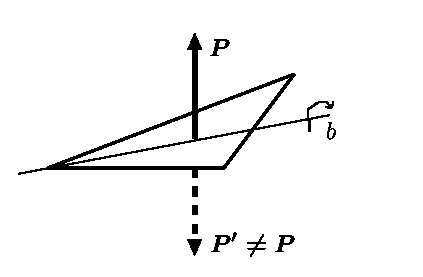
\includegraphics[scale=1.0]{pics/nodipol.eps}}

Simetrični kristal ne može "proizvesti" nesimetrični dipolni moment.

Grupno-teorijski iskaz ovog: \emph{Reprezentacija grupe $G$ na vektorskom
prostoru (potencijalnih) vektora dipolnog momenta mora biti trivijalna tj.
identiteta}:
\begin{displaymath}
   D(g)=1 \quad \forall g\in G \;.
\end{displaymath}
Dakle, da bi kristal mogao imati $\vec{P}\neq 0$, reprezentacija grupe $G$ na 
3D euklidskom vektorskom prostoru mora 
u svojoj dekompoziciji na IRREPse sadržavati identitetu.

Vidjeli smo u prošlom odjeljku da je REP $\Gamma_V$ od $D_3$ na 3D
euklidskom vektorskom prostoru
\begin{displaymath}
             \Gamma_V = A_2 \oplus E \;.
\end{displaymath}
Nema $A_1$ (identitete) $\imp$ nema dipolnog momenta.

S druge strane, za $C_3$ imamo (D.Z.)
\begin{displaymath}
             \Gamma_V = A_1 \oplus E \;.
\end{displaymath}
$\imp$ postoji mogućnost dipolnog momenta.

\textbf{Aksijalni vektori}

Kad grupa pored rotacija sadrži i refleksije ($\sigma$, $S_n$, $i$) treba
uzeti u obzir činjenicu da je magnetski moment $\vec{M}$ aksijalni
vektor (vidi Dodatak \ref{sec:aksijalni})
koji se pri takvim transformacijama ponaša obrnuto od običnog
(polarnog) vektora električnog dipolnog momenta:

\centerline{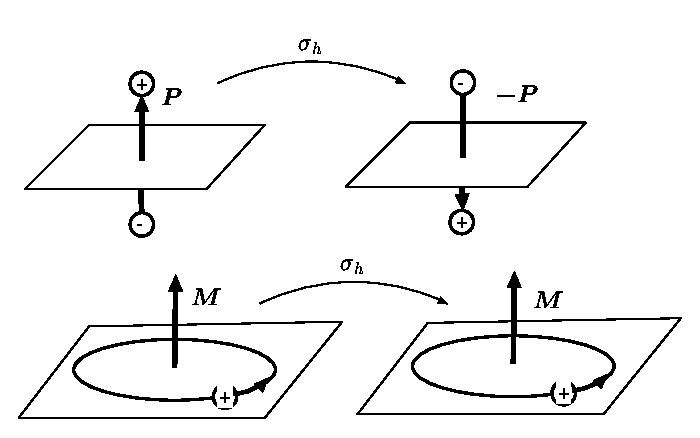
\includegraphics[scale=0.8]{pics/aksijal1.eps}}

\centerline{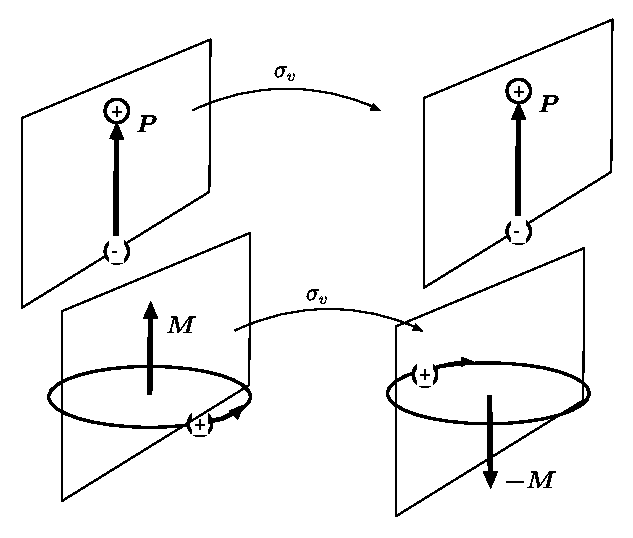
\includegraphics[scale=0.8]{pics/aksijal2.eps}}

(D.Z. Razmislite zašto ogledalo izvrće lijevo-desno, a ne i gore-dolje? kad je
$\sigma_{v_{\mbox{\tiny ogledalo u $x-z$ ravnini}}}:(x, y, z)\to (x, -y, z)$?)

\begin{primjer}[Kristal s $C_{3v}$ simetrijom]

Grupa $C_{3v}$ je izomorfna grupi $D_3$, jedino što $b$ nije rotacija
za $\pi/2$ oko horizontalne osi već refleksija oko vertikalne ravnine
koja sadrži $C_3$ os.

Reprezentacija elemenata $e, c$ i  $c^2$ je kao na strani \ref{pgC3matrice},
\begin{displaymath}
D(c)=
\left(
\begin{array}{ccc}
-1/2 & -\sqrt{3}/2 & 0 \\
\sqrt{3}/2 & -1/2 & 0 \\
0 & 0 & 1
\end{array}\right) \;, \ldots
\end{displaymath}
s karakterima $\chi^{V}(e)=\mbox{dim}\Gamma_{V}=3$, $\chi^{V}(c)=0$,
a ako osi izberemo kao na slici
\centerline{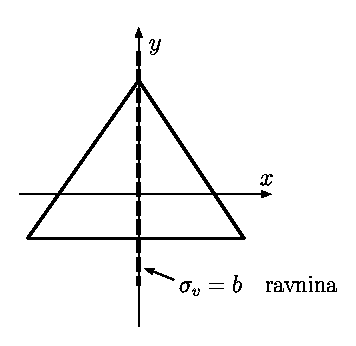
\includegraphics[scale=0.8]{pics/C3vravnina.eps}}
onda je 

\begin{displaymath}
D^{V}(b)=
\left(
\begin{array}{ccc}
-1 & 0 & 0 \\
0 & 1 & 0 \\
0 & 0 & 1
\end{array}\right) 
\end{displaymath}
s karakterom $\chi^{V}(b)=1$.

(Za $D_3$  grupu bi bilo $D^{V}(b)=diag(-1, 1, -1)$, s karakterom
$\chi^{V}(b)=-1$.)

Kako je grupa izomorfna grupi $D_3$ ima istu tablicu karaktera (usput, obrat
ne vrijedi, $Q$ i $T_d$ imaju iste tablice, a nisu izomorfne). Dakle,
imamo:

\begin{tabular}{c|ccc}
  & E & 2$C_3$  & 3$C_2$ \\ \hline
$A_1$ & 1 & 1& 1 \\
$A_2$ & 1 & 1&-1 \\
 $E$  & 2 &-1& 0 \\ \hline
 $\Gamma_V$ & 3 & 0 & 1
\end{tabular}

Iz ovog onda slijedi
\begin{displaymath}
   \Gamma_{V} = A_1  \oplus E
\end{displaymath}

- U rastavu se javlja $A_1$ $\imp$ moguć je permanentni \emph{električni}
 dipolni
moment.


Za aksijalne vektore, reprezentacije elemenata $e, c, c^2$ su iste kao i
gore, ali za $D^{A}(b)$ imamo suprotno od $D^{V}(b)$:

\begin{displaymath}
D^{A}(b)=
\left(
\begin{array}{ccc}
1 & 0 & 0 \\
0 & -1 & 0 \\
0 & 0 & -1
\end{array}\right) 
\end{displaymath}
s karakterom $\chi^{A}(b)=-1$.
(Oblik matrice se može naći i iz razmatranja djelovanja $\sigma_{v}$ na
aksijalni vektor $\vec{c}=\vec{a}\times\vec{b}$ gdje 
su $\vec{a}$ i $\vec{b}$ pravi
vektori: $\sigma_{v}:(a_x, a_y, a_z)\to (-a_x, a_y, a_z)$,
 $\sigma_{v}:(b_x, b_y, b_z)\to (-b_x, b_y, b_z)$
$\imp$  $\sigma_{v}:(c_x, c_y, c_z)\to (c_x, -c_y, -c_z)$.)

Dakle, ukupni karakter je $\chi^{A}=(3, 0, -1)$ odnosno
\begin{displaymath}
      \Gamma_{A} = A_2 \oplus E
\end{displaymath}

Tu nema identitete $A_1$ pa ne može biti ni permanetnog \emph{magnetskog}
dipolnog momenta.
\end{primjer}

\section{Primjena: \emph{Degeneracija i cijepanje energijskih nivoa}}
\label{degeneracija}

Transformacije u kvantnoj mehanici:
\begin{align*}
 \psi' &= U \psi \qquad &\text{za stanja --- vektore} \\
   A' &= U^{-1} A U \qquad &\text{za operatore}
\end{align*}
$U$ --- operator transformacije. Kvantnomehanički sustav, zadan
hamiltonijanom $H_0$, je \emph{simetričan} obzirom na skup transformacija
$\{ U(g_1), U(g_2), \ldots, U(g_n)\}$ ako transformacije ne mijenjaju
hamiltonijan (on, možemo reći, putem Schr\"{o}dingerove jednadžbe definira ``izgled"
sustava)
\begin{displaymath}
U^{-1}(g) H_{0} U(g) = H_{0} \quad \forall  g \in \{g_1,\ldots, g_n\}\;.
\end{displaymath}
Ekvivalentno, tada $U(g)$ i $H_0$ komutiraju:
\begin{displaymath}
  H_{0}U(g)=U(g)H_0 \quad \forall  g \in \{g_1,\ldots, g_n\} \;.
\end{displaymath}
Skup svih operatora s ovim svojstvom čini grupu (provjerite!) tj.
reprezentaciju grupe $G=\{g_1,\ldots, g_n\}$ na prostoru kvantnomehaničkih 
stanja.

Stanje sustava s dobro definiranom energijom $\psi_n(\vec{x})$ zove se
\emph{stacionarno stanje} i dano je kao rješenje vremenski 
neovisne Schr\"{o}dingerove jednadžbe
\begin{displaymath}
  H_0 \psi_n(\vec{x}) = E_n \psi(\vec{x}) \;.
\end{displaymath}
Energija transformiranih stanja $\psi'_n(\vec{x}) = U(g)\psi_n(\vec{x})$ je
odgovarajuća svojstvena vrijednost hamiltonijana
\begin{displaymath}
  H_0 \psi'_n(\vec{x}) = H_0 U(g)\psi_n(\vec{x}) = U(g) H_0 \psi_n(\vec{x}) =
 U(g) E_n \psi_n(\vec{x}) = E_n \psi'_n(\vec{x}) \;.
\end{displaymath}
Dakle sva stanja $\psi'_n(\vec{x}) = U(g)\psi_n(\vec{x})$, $\forall g$ imaju
istu energiju $E_n$. Pojavu kad više stanja ima istu energiju 
nazivamo \emph{degeneracija}.

Skup stanja $\{U(g)\psi_n(\vec{x}) \,|\, g\in G\}$ dobivenih transformacijama
datog stanja $\psi_n(\vec{x})$ razapinje
potprostor vektorskog prostora svih stanja sustava. On je
po definiciji invarijantan na djelovanje reprezentacije $\{ U(g) \}$.
Također, reprezentacija $\{ U'(g) \}$ dobivena redukcijom reprezentacije
$\{ U(g) \}$ na ovaj potprostor je ireducibilna što slijedi
iz načina na koji smo konstruirali potprostor.
Takav potprostor naziva se \emph{multiplet}\footnote{Često ze izraz
multiplet koristi i za samu bazu ovog potprostora.}.

Dakle, poznavajući sve IRREPse grupe simetrija nekog kvantnomehaničkog
sustava možemo odrediti mogućnosti degeneracije njegovih stanja ---
one su jednake dimenzionalnostima IRREPsa.

\begin{primjer}[oktahedralna grupa O]

- IRREPsi: $\underbrace{A_1, A_2}_{1D}, \underbrace{E}_{2D},
            \underbrace{T_1, T_2}_{3D}$

- $\imp$ očekujemo jedno-, dvo- i trostruko degenerirane nivoe.

\hspace*{2cm}
\rule{3cm}{1pt}\hspace*{-3cm}%
\rule[2pt]{3cm}{1pt}\hspace*{-3cm}%
\rule[4pt]{3cm}{1pt}\hspace{12pt}%
$\psi_{T_1,1}, \psi_{T_1,2}, \psi_{T_1,3}$

\hspace*{2cm}
\rule{3cm}{1pt}\hspace*{12pt}%
$\psi_{A_2}'$

\hspace*{2cm}
\rule{3cm}{1pt}\hspace*{12pt}%
$\psi_{A_1}$

\hspace*{2cm}
\rule{3cm}{1pt}\hspace*{-3cm}%
\rule[2pt]{3cm}{1pt}\hspace*{12pt}%
$\psi_{E,1}, \psi_{E,2}$

\hspace*{2cm}
\rule{3cm}{1pt}\hspace*{12pt}%
$\psi_{A_2}$

$\psi_{A_2}'$ i $\psi_{A_2}$ su linearno neovisne funkcije.
Pronađemo li neki nivo s prevelikom degeneracijom,
npr\\

\hspace*{2cm}
\rule{3cm}{1pt}\hspace*{-3cm}%
\rule[2pt]{3cm}{1pt}\hspace*{-3cm}%
\rule[4pt]{3cm}{1pt}\hspace{12pt}%
$\psi_{E,1}, \psi_{E,2}, \psi_{A_1}$

to gotovo uvijek znači da nismo dobro identificirali grupu simetrija
tj. da sustav ima veću simetriju nego što smo mislili.

\end{primjer}


\begin{primjer}[Vodikov atom]

Stacionarna stanja su $\psi_{nlm}(\vec{x})$. G=SO(3) --- sferna simetrija.
U 6. poglavlju ćemo vidjeti da su multipleti oblika
\begin{displaymath}
   \{ \psi_{nl(-l)}, \psi_{nl(-l+1)}, \ldots, \psi_{nll}\} \qquad 
\text{($2l+1$ stanja)} \;.
\end{displaymath}
$\imp$ očekujemo $(2l+1)$-struko degenerirane nivoe za svaki $l$. No,
znamo da je zapravo degeneracija $n^2$-struka. Svaka ljuska ima $n^2$
stanja energije
\begin{displaymath}
  E_n \propto \frac{1}{n^2} \qquad \text{neovisno o $l$}
\end{displaymath}
``Slučajna'' degeneracija nivoa s različitim $l$. U 6. poglavlju
ćemo vidjeti da je razlog tome 
postojanje veće simetrije SO(4)=SO(3)$\otimes$SO(3).
\end{primjer}

\subsection*{Cijepanje energijskih nivoa}

Zamislimo sada da neka smetnja $V$  promijeni hamiltonijan
\begin{displaymath}
    H_0 \to H = H_0 + V \;,
\end{displaymath}
tako da je ukupni hamiltonijan $H$ invarijantan na manju grupu $H<G$.
(Npr. slabo električno polje u Starkovom efektu mijenja Hamiltonijan
vodikovog atoma tako da mu doda član proprocionalan električnom polju
i od originalne sferne simetrije preostaje samo aksijalna.)

IRREPsi od $G$ nisu nužno i IRREPsi od $H$. Smanjenje broja transformacija
$U(h)$, $h\in H$ može učiniti da neki potprosotri postanu invarijantni
iako nisu bili invarijantni na potpun skup transformacija $U(g)$, $g\in G$.
Tako su neke IRREPs od G reducibilne obzirom na H i nema razloga da 
nivoi koji odgovaraju dotičnim IRREPsima od G ostanu
degenerirani

\centerline{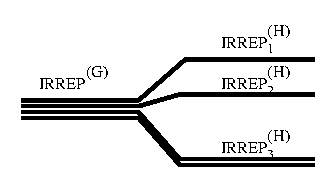
\includegraphics[scale=1.0]{pics/splitting.eps}}
 
Poznavajući dekompoziciju $IRREP^{(G)}$ na $IRREP^{(H)}$
\begin{displaymath}
   IRREP^{(G)}=(\text{reducibilna REP})^{(H)}=
 IRREP^{(H)}_1 \oplus IRREP^{(H)}_2 \oplus \cdots
\end{displaymath}
možemo odrediti strukturu cijepanja. Za određivanje iznosa cijepanja
koriste se metode kvantnomehaničkog računa smetnje.

\begin{primjer}[Cijepanje $T$-nivoa tetrahedralne grupe $T$]

Karakter $T$-nivoa tetrahedralne grupe je
\begin{displaymath}
\begin{tabular}{c|cccc}
  & E & 3$C_2$  & 4$C_3$ & 4$C_{3}'$ \\ \hline
 $T$ & 3  & -1 & 0 & 0 
\end{tabular}
\end{displaymath}

Neka npr. sada kristal doživi fazni prijelaz tako da se
simetrija smanji a) $T\to D_2$ ili b) $T\to C_{3v}$. Pogledajmo
što se događa s gornjim četverostruko degeneriranim nivoom.

a)

\begin{displaymath}
\begin{tabular}{c|cccc}
 & $E$  & $C_{2}^z$ &  $C_{2}^y$ & $C_{2}^x$ \\ \hline
$A_1$ & 1 & 1& 1 & 1 \\
$B_1$ & 1 & 1&-1  & -1\\
$B_2$ & 1 & -1&1  & -1\\
$B_3$ & 1 & -1&-1  & 1\\ \hline \hline
 $T$ & 3 & -1 & -1 & -1
\end{tabular}
\end{displaymath}

Uobičajenim metodama dekompozicije reducibilnih reprezentacija
dobivamo:
\begin{displaymath}
   T = a_1 A_1 \oplus b_1 B_1 \oplus b_2 B_2 \oplus b_3 B_3
\end{displaymath}

\begin{align*}
a_1 &= \frac{1}{n}\sum_k \chi^{(A_1)}(k) \chi^{(T)^*}(k) =
 \frac{1}{4}\big(1\cdot3 + 1\cdot(-1) + 1\cdot(-1) + 1\cdot(-1)\big) = 0 \\
b_1 =b_2 = b_3 &= 1
\end{align*}
\begin{displaymath}
  \imp   T =  B_1 \oplus B_2 \oplus B_3
\end{displaymath}
Dakle degeneracija je potpuno ukinuta

\centerline{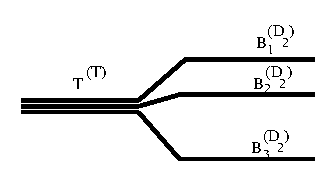
\includegraphics[scale=1.0]{pics/splittingT.eps}}

b) Isti postupak daje
\begin{displaymath}
        T = A_2 \oplus E \;,
\end{displaymath}
tj. degeneracija je samo djelomično ukinuta.

\centerline{\includegraphics[scale=1.0]{pics/splittingT2.eps}}

\end{primjer}

\section{Dodatak: \emph{Kristalografske oznake}}

\textbf{Ireducibilne reprezentacije} $\Gamma^{(\alpha)}$ se obično označavaju
velikim slovima i to tako da se 1D reprezentacije označavaju slovima
$A$ i $B$, 2D reprezentacije slovom $E$, 3D reprezentacije slovom $T$
itd. Par kompleksno konjugiranih 1D reprezentacija se smatra jednom
2D reprezentacijom (jer ih povezuje vremenska inverzija) tako da se
one udružuju vitičastom zagradom i označavaju s $E$.

\textbf{Klase konjugacije} se obično označavaju simbolom $mC_n$ gdje je $m$
broj elemenata klase, a $C_n$ tipični predstavnik klase označen
Sch\"{o}nfliesovim simbolom:

\begin{tabular}{rcl}
$E$ & = & identiteta \\
$C_n$ & = & rotacija za $2\pi/n$ \\
$\sigma$ & = & refleksija preko ravnine \\
$\sigma_{h}$ & = & refleksija preko ``horizontalne'' ravnine tj. ravnine
  okomite da os najveće  \\ && rotacijske simetrije \\
$\sigma_{v}$ & = & refleksija preko ``vertikalne'' ravnine tj. ravnine
  koja sadrži os najveće \\ &&rotacijske simetrije \\
$\sigma_{d}$ & = & refleksija preko ``dijagonalne'' ravnine tj. ravnine
  koja sadrži os najveće \\ && rotacijske simetrije i raspolavlja kut između
  dvije $C_2$ osi okomite na tu os. \\ &&(Specijalni slučaj $\sigma_{v}$.) \\
$S_n$  & = & rotacija za $2\pi/n$ kombinirana s refleksijom preko ravnine
   okomite na \\ && os te rotacije (Ove dvije operacije komutiraju.) \\
$i$ & = &  $S_2 \;\, = \;\,$  inverzija $\vec{r} \to -\vec{r}$
\end{tabular}

\textbf{Točkaste grupe} kristala se označavaju slijedećim
Sch\"{o}nfliesovim oznakama:

\begin{tabular}{rcl}
$C_n$ & = & grupe s jednom $C_n$ osi simetrije \\
$C_{nv}$ & = & grupe s jednom $C_n$ osi i $n$ $\sigma_v$
   refleksijskih ravnina  \\
$C_{nh}$ & = & $C_n$ os,  $\sigma_h$ refleksija $+$ dodaci \\
$S_{n}$ & = & $S_n$ os \\
$D_{n}$ & = & $C_n$ os i $n$ $C_2$ osi okomitih na nju \\
$D_{nd}$ & = & elementi od $D_{n}$ i $\sigma_d$ ravnine refleksije \\
$D_{nh}$ & = & elementi od $D_{n}$ i $\sigma_h$ ravnina refleksije \\
$T$  & = & tetrahedralna grupa \\
$O$  & = & oktahedralna grupa \\
$\cdots$ && $\cdots \quad$ itd. vidi literaturu \\
\end{tabular}

\section{Dodatak: \emph{Aksijalni vektori (pseudovektori)} \label{sec:aksijalni}}
\label{sec:pseudovektori}

\emph{Aksijalni} ili \emph{pseudovektori} su objekti koji se pri rotacijama transformiraju
isto kao i obični (tzv. \emph{polarni}) vektori, ali pri refleksijama i inverzijama
imaju još i dodatnu promjenu predznaka.

Inverzija običnim vektorima u 3D euklidskom prostoru mijenja
predznak $i: \vec{r} \to - \vec{r}$ i može se reprezentirati dijagonalnom
matricom $i = -\Eins = {\rm diag}(-1, -1, -1)$. 

No, vektorski produkt dvaju polarnih vektora, npr. vektora položaja $\vec{r}$
i impulsa $\vec{p}$ posljedično \emph{ne mijenja} predznak:

\[  \vec{L}\equiv \vec{r}\times\vec{p} \; \stackrel{i}{\longrightarrow} \;
  (-\vec{r}) \times (-\vec{p}) =  \vec{r}\times\vec{p} = \vec{L}  \;,
\]

što znači da je $\vec{L}$ (moment impulsa) aksijalni vektor. (U fizici su
veličine koje opisuju rotacije, poput momenta impulsa ili momenta sile, 
često reprezentirane aksijalnim vektorima. Isto vrijedi za veličine
vezane uz magnetizam koji je obično rezultat kruženja (mikro ili makro) struja.)

Da bi se naglasila njihova različitost,
ponegdje u literaturi se aksijalne vektore ne crta kao usmjerene crte
(strelice), već kao crte s ``aksijalnim strelicama'' (cf. 
\cite{Bronstejn04} p. 186)

\centerline{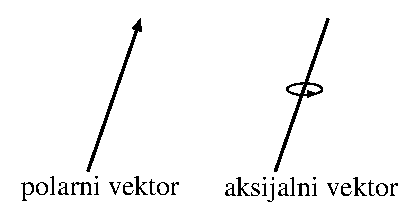
\includegraphics[scale=0.8]{pics/aksijalni_vektor.eps}}

Slično definiramo \emph{pseudoskalarne} veličine kao one koje su skalari
obzirom na rotacije, ali mijenjaju predznak pri refleksijama i inverzijama.
Npr. miješani produkt polarnih vektora je pseudoskalar:

\[
P = (\vec{r}_1 \times \vec{p}) \cdot \vec{r}_2  \; \stackrel{i}{\longrightarrow} \;
  - (\vec{r}_1 \times \vec{p}) \cdot \vec{r}_2 = - P
\]

Magnetski moment, definiran kao $\vec{M} = \frac{1}{2} \int \vec{r}
\otimes \vec{J} dV$ za gustoću struje $J$, odnosno kao
$\vec{M} = \frac{1}{2} q \vec{r} \otimes \vec{v}$ za točkasti
naboj $q$, je dakle aksijalni vektor.

Za još detalja o pseudovektorima i drugim pseudo-veličinama vidi
npr. \cite{Arfken95}.

\subsection*{Zadaci}

\begin{enumerate}[{3}.1]

\item Konstruirajte 2D IRREP grupe $D_3$ koja djeluje na $x-y$ ravnini
i provjerite temeljni teorem o ortogonalnosti.

\item Pokažite da su sve IRREP Abelovih grupa jednodimenzionalne.

\item Pokažite da je nužan i dovoljan uvjet ireducibilnosti reprezentacije
 $\Gamma$ s karakterima $\chi_i$ tzv. Frobeniusov kriterij
\begin{displaymath}
    \sum_i k_i |\chi_i|^2 = n  \;,
\end{displaymath}
gdje je $k_i$ broj elemenata u klasi konjugacije $i$.

\item Konstruirajte tablicu karaktera za grupu $D_4$

\item Pokažite da je direktni produkt dvije 1D IRREP uvijek IRREP.

\item Izrazite reprezentaciju $\Gamma$ grupe $C_{4v}$ koja ima
karaktere
\begin{displaymath}
  \chi(E)=5\;,\quad \chi(C_2)=1\;,\quad \chi(C_4)=-1\;,\quad
  \chi(\sigma_v)=1\;,\quad \chi(\sigma_d)=-3\;,
\end{displaymath}
kao zbroj IRREPsa.
\end{enumerate}

